\documentclass[12pt, a4paper]{article}
\usepackage[english]{babel}

% margins
\usepackage[a4paper, margin=2.5cm]{geometry}

% include pdf
\usepackage[final]{pdfpages}

% fix line breaks urls
\PassOptionsToPackage{hyphens}{url}
\usepackage[hidelinks]{hyperref}

\usepackage{graphics}

% Special/larger tables
\usepackage{longtable}
\usepackage{tabularx}

% Centered X
\newcolumntype{Y}{>{\centering\arraybackslash}X}
% Centered p
\newcolumntype{P}[1]{>{\centering\arraybackslash}p{#1}}

% quotes
\usepackage{csquotes}

% Numbers and SI units
\usepackage{siunitx}
\sisetup{
  group-four-digits = true,
  group-separator = {,}
}


% Acronyms
\usepackage[nopostdot,style=super,nonumberlist,toc,nogroupskip,acronym]{glossaries}

% Double spacing
\usepackage{setspace}

% appendix
\usepackage[page, title]{appendix}

% tables
\usepackage{booktabs}
\usepackage{array} % centering + width fix

\usepackage{caption} 
\captionsetup{labelfont=bf,labelsep=period,font=small} 
\usepackage{cleveref}

% Times New Roman
%\usepackage{newtxtext,newtxmath}

% Page numbering right
\usepackage{fancyhdr}
\pagestyle{fancy}
% Clear the header and footer
\fancyhead{}
\fancyfoot{}
\renewcommand{\headrulewidth}{0pt}
% Set the right side of the footer to be the page number
\fancyfoot[R]{\thepage}

% Fix section titles size/format
\usepackage{titlesec}
\titleformat{\section}
  {\normalfont\fontsize{16}{19.2}\bfseries}
  {\thesection}
  {1em}
  {}

\titleformat{\subsection}
  {\normalfont\fontsize{14}{17}\bfseries}
  {\thesubsection}
  {1em}
  {}

  \titleformat{\subsubsection}
  {\normalfont\fontsize{12}{14}\itshape} 
  {\thesubsubsection}
  {1em}
  {}

\titlespacing{\section}{0pt}{\parskip}{-\parskip}
\titlespacing{\subsection}{0pt}{0.75\parskip}{-\parskip}
\titlespacing{\subsubsection}{0pt}{0.5\parskip}{-\parskip}

% Remove section numbers
\setcounter{secnumdepth}{0}

% Set paragraph spacing
\setlength{\parindent}{0pt}
\setlength{\parskip}{1em}
\def\ni{\noindent}

%% These two lines are needed to get the correct paper size
%% in TeX Live 2016
\let\pdfpageheight\paperheight
\let\pdfpagewidth\paperwidth

\makenoidxglossaries

\newacronym{auc}{AUC}{area under the receiver operating characteristic curve}
\newacronym{mam}{M\&M}{morbidity and mortality}
\newacronym{ml}{ML}{machine learning}
\newacronym{ofi}{OFI}{opportunity for improvement}
\newacronym{qi}{QI}{quality improvement}
\newacronym{gan}{GAN}{generative adversarial network}
\newacronym{iss}{ISS}{injury severity score}
\newacronym{swetrau}{SweTrau}{Swedish Trauma Registry}
\newacronym{ci}{CI}{confidence interval}
\newacronym{ctgan}{CTGAN}{conditional tabular generative adversarial network}
\newacronym{tvae}{TVAE}{triplet based variational autoencoder}
\newacronym{vae}{VAE}{variational variable autoencoder}
\newacronym{sd}{SD}{standard deviation}

\newglossaryentry{trauma}
{
    name=Trauma,
    text=trauma,
    description={The clinical entity composed by physical injury and the body's associated response. \cite{gerdin_risk_2015}} 
}

\newglossaryentry{gofi}
{
    name={OFI},
    text={OFI},
    description={Short for opportunity for improvement, is a consensus reached at a morbidity and mortality conference regarding whether there exists opportunity for improvement in the handling of a singular patient trauma care.}
}



% Acronym style
\newglossarystyle{csuper}{%
    \setglossarystyle{super}%
    \renewcommand{\glossentry}[2]{%
        \glsentryitem{##1}\glstarget{##1}{\glossentryname{##1}} &
        \Glossentrydesc{##1}\glspostdescription\space ##2\tabularnewline
    }
    \setlength{\glsdescwidth}{0.75\linewidth}
}

% Glossary style
\newglossarystyle{gsuper}{%
    \setglossarystyle{super}%
    \renewcommand{\glossentry}[2]{%
        \glsentryitem{##1}\glstarget{##1}{\glossentryname{##1}} &
        \Glossentrydesc{##1}\glspostdescription\space ##2\\[1em]
    }
    \setlength{\glsdescwidth}{0.65\linewidth}
}

% References
\usepackage[style=numeric,
    backend=biber,
    sorting=none,
    url=false,
    isbn=false,
    terseinits=true,
    giveninits=true,
    minnames=6,
    maxnames=6]{biblatex}

% Remove unwanted punctuations
\renewcommand*{\revsdnamepunct}{}
\renewcommand*{\finentrypunct}{}
\renewcommand*{\bibpagespunct}{}

% Dot instead av brackets in references
\DeclareFieldFormat{labelnumberwidth}{\mkbibbold{#1\adddot}}

% Lastname followed by initials format
\DeclareNameAlias{sortname}{family-given}
\DeclareNameAlias{default}{family-given}
\renewcommand*{\revsdnamepunct}{}

\DeclareSourcemap{%
    \maps[datatype=bibtex]{
        % Journal abbreviations
        \map[overwrite]{
            \step[fieldsource=shortjournal]
            \step[fieldset=journaltitle,origfieldval]
        }
    }
}

% remove in
\renewbibmacro{in:}{}
% remove pp
\DeclareFieldFormat*{pages}{#1}
% reformat doi
\DeclareFieldFormat*{doi}{\url{https://doi.org/#1}}
%remove quotation marks around title
\DeclareFieldFormat*{title}{#1}


\DeclareFieldFormat{journaltitle}{\mkbibemph{#1}\isdot}

% Provide three letter month names
\newcommand*{\shortmonth}[1]{
    \ifthenelse{\NOT\equal{#1}{}}{
        \ifcase#1\relax
        \or Jan
        \or Feb
        \or Mar
        \or Apr
        \or May
        \or Jun
        \or Jul
        \or Aug
        \or Sep
        \or Oct
        \or Nov
        \or Dec
        \fi
    }
}

\DeclareFieldFormat*{number}{\mkbibparens{#1}}

\DeclareFieldFormat*{date}{\thefield{year}}

% Code adapted from biblatex-nejm package

\renewbibmacro*{volume+number+eid}{
    \printfield{volume}%
    \setunit{}%
    \printfield{number}%
    \addcolon%
    \printfield{eid}%
}

\renewbibmacro*{issue+date}{
    \usebibmacro{date}
}

\renewbibmacro*{journal+issuetitle}{
    \usebibmacro{journal}%
    \iffieldundef{series}%
    \adddot%
    {}
    {\newunit%
        \printfield{series}}%
    \setunit{\addspace}%
    \usebibmacro{issue+date}%
    \setunit{\addsemicolon}%
    \usebibmacro{volume+number+eid}%
    \usebibmacro{issue}%
    \newunit}

% compress page numbers. E.g. XYZ-XAB -> XYZ-AB
\DeclareFieldFormat{postnote}{\mkcomprange[{\mkpageprefix[pagination]}]{#1}}
\DeclareFieldFormat{pages}{\mkcomprange{#1}}

% Compress ranges where lower limit > 100
\setcounter{mincomprange}{100}

% Don't compress beyond the fourth digit
\setcounter{maxcomprange}{1000}

% Display compressed upper limit with at least two digits,
% unless leading digit is zero
\setcounter{mincompwidth}{10} %imports biblatex 
\addbibresource{main.bib}


\begin{document}
\pagenumbering{Roman}

\begin{titlepage}
    
\includepdf[pages=-,pagecommand={},fitpaper=true,]{title_page.pdf}
\end{titlepage}
\setstretch{1}
\fontsize{11}{13}\selectfont

\addcontentsline{toc}{section}{Abstract}

\textbf{Titel}

\vfill

\textbf{Title}

\vfill

\textit{Keywords}: Machine learning; Trauma; Medical audit; Trauma care quality improvement; Data synthesis; Prediction

\newpage

\normalsize

\glsaddall
\printnoidxglossary[type=acronym,style=csuper]
\printnoidxglossary[style=gsuper]

\newpage
\pagenumbering{arabic}

\setstretch{1.45}

\section{Introduction}
\Gls{trauma} is a significant contributor to mortality and morbidity for people between the ages of 10 and 49 globally, and it is the leading cause of death among young people in Sweden \cite{roth_global_2018, vos_global_2020, sos_death_2021}. The average age of the trauma population is low, and two-thirds of this group have no previous history of co-morbidity \cite{brattstrom_socio-economic_2015}. As a result, it is crucial to provide high-quality trauma care to reduce mortality and morbidity rates for this population, which has a long-life expectancy. The estimated age standardised disability-adjusted life years for the population is 247.6 million, compared to the most common cause of mortality globally, ischaemic heart disease, with 170.3 million years \cite{haagsma_global_2016,wang_global_2021,roth_global_2018}.

One way to enhance trauma patient care is through the implementation of \acrfull{qi} programs, as recommended by the World Health Organization (WHO) \cite{world_health_organization_guidelines_2009}. These \acrshort{qi} programs have a base in the three concepts for quality assurance suggested by Donabedian - structure, process, and outcomes \cite{donabedian_effectiveness_1996}. \Acrfull{mam}  conferences are a crucial component of these programs and aim to identify \acrfull{ofi} in patient care \cite{santana_development_2014}. \acrshort{mam} conferences are conducted by representatives from all disciplines and professions involved in trauma care, during which the treatment provided to an individual patient is evaluated and compared to the optimal treatment that should have been provided. Regularly conducting these reviews is linked to a reduction in complication rates, hospital stay time, and preventable deaths, thereby providing high-quality trauma care \cite{stelfox_evidence_2011, mcdermott_trauma_1994}. The conferences aim to address all pillars suggested by Donabedian for quality assurance, however, due to their nature, \acrshort{mam} conferences are highly resource-intensive.

An \acrshort{ofi}, identified by an \acrshort{mam} conference, refers to a specific deficit in patient care and often occurs in initial care, including airway management, fluid resuscitation, haemorrhage control, and chest injury management \cite{world_health_organization_guidelines_2009,roy_learning_2017,oreilly_opportunities_2013,sanddal_analysis_2011}. The incidence of \acrshortpl{ofi} for both morbidity and mortality patients has not been well researched, however, at Karolinska University Hospital the incidence for \acrshortpl{ofi} in the trauma population is at 7\% \cite{attergrim_predicting_2023}. In other words, if all trauma patients were brought up at a \acrshort{mam}, fourteen in fifteen cases would not result in an \acrshort{ofi} being found.

Therefore, a more advanced \acrshort{qi} technique suggested by World Health Organization is the application of audit filters that use electronic health record systems to monitor predefined variables to flag patient cases with potential \acrfull{ofi} \cite{world_health_organization_guidelines_2009}. Filtering cases with an audit filter system before reviewing by an \acrshort{mam} conference provides a possibility to reduce false positive cases and thus reducing the costs of the \acrshort{qi} programme as a whole.

However, the performance of these systems is inconsistent and has been linked to high rates of false positives. Depending on the context, the frequency of false positives can range from 24\% to 80\% \cite{attergrim_predicting_2023,sanddal_analysis_2011,roy_learning_2017,ghorbani_analysis_2018}. It has been suggested to use calculated probability of survival (PS) and Trauma Score and Injury Severity Score (TRISS) as audit filters. TRISS and PS have a poor track record in detecting a substantial number of preventable deaths and miss important \acrshort{ofi} \cite{heim_survival_2016}.

A newer approach proposed by Attegrim and Szolnoky et al. \cite{attergrim_predicting_2023} recommends replacing audit filter systems with supervised \acrfull{ml} models. These newer models exhibit a significantly improved performance compared to the audit filter system currently used at Karolinska University Hospital in Stockholm, Sweden. When maintaining the same sensitivity, the false positive rate was reduced from 68\% to 53\% with the use of the same data. \acrshort{ml} in trauma has existed for some time and most studies investigate the application of \acrshort{ml} models in prediction mortality and complications \cite{zhang_machine_2022}. This is the first time that \acrshort{ml} models have been used to predict \acrshort{ofi} in trauma care.

The models investigated by Attegrim and Szolnoky et al. include traditional \acrshort{ml} methods: logistic regression, random forest \cite{breiman_random_2001}, decision trees, support vector machines \cite{cortes_support-vector_1995}, as well as newer boosting models: XGBoost \cite{chen_xgboost_2016}, LightGBM \cite{ke_lightgbm_2017}, and CatBoost \cite{prokhorenkova_catboost_2018}. The overall best performing model was LightGBM.

Despite the improved performance, the models still have a problem in that 50\% of patient cases are inaccurately marked as \acrshort{ofi} positive. \acrshort{ml} methods generally require substantial amounts of data to perform effectively \cite{piccialli_survey_2021}. There are several ways to enhance the performance of \acrshort{ml} models, and the most basic and well-known is simply increasing the amount of data. Until now, the only option for doing so was by manually gathering more data and annotating it. This process is slow, and in some cases, not feasible due to a shortage of data.

% \begin{figure}
%     \centering
%     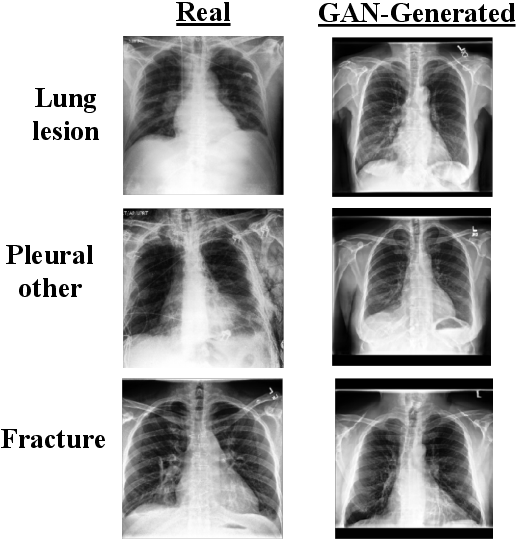
\includegraphics[width=0.6\textwidth]{figures/gan-xray.png}
%     \caption{Example of using a \acrfull{gan} to generate chest radiograph images. Image taken from \cite{sundaram_gan-based_2021}.}
%     \label{fig:gan-xray}
% \end{figure}
% See \Cref{fig:gan-xray} for an example usage of \acrshortpl{gan} in image analysis.

Recently, the use of \acrfullpl{gan} to generate synthetic data has become a popular topic in image analysis \cite{pavan_kumar_generative_2021}.  A \acrshort{gan} is a type of artificial neural network consisting of two main components: a generator and a discriminator. The generator is trained to produce new data samples that resemble the input data, while the discriminator is trained to differentiate between the generated samples and the real data.

The generator and discriminator are trained together in an adversarial manner. The generator aims to produce samples that the discriminator cannot identify as fake, while the discriminator strives to accurately identify the fake samples generated by the generator. This process allows the generator to learn to produce samples that resemble the input data, and the discriminator to learn to distinguish between real and generated data. As a result, the generator continually improves, producing data that more closely resembles the source and becomes increasingly difficult for the discriminator to identify as synthetic data.

In addition to generating more trainable data, some \acrshortpl{gan} are able to anonymise data \cite{liu_ppgan_2019} and provide an interface for being able to generate synthetic datasets of sensitive personal information that are completely anonymous. These synthetic datasets can, in theory, be distributed and increase the availability of medical datasets for researchers.

Another type of generative model in artificial neural networks is the \acrfull{vae} \cite{kingma_auto-encoding_2013}. It is a simpler and more compact model that learns the probabilistic representation of a dataset, called the latent space. This representation is a compressed form of the input data that captures its most important features and variations. The \acrshort{vae} consists of two parts: an encoder and a decoder. The encoder maps the input data to a probability distribution in the latent space, while the decoder maps a sample from that distribution back to the original data space. By training the \acrshort{vae}, we learn a compact representation of the input data that highlights its important features and variations.

The quality of the generated data from these methods often varies and is dependent on several factors, such as the quality and quantity of the ground truth data \cite{karras_training_2020}.  The major advantage of having a method for generating high-quality synthetic data is the ability to enlarge small datasets and train \acrshort{ml}  models in cases where it was not feasible before, or did not produce satisfactory results due to a lack of data. This has been previously explored in medical image analysis contexts where it has also been shown to improve cross-site generalisation \cite{sanaat_robust-deep_2022, bashyam_deep_2022}.

However, the use of \acrshortpl{gan} and \acrshortpl{vae} for structured tabular data is relatively uncommon and largely unexplored. There are few studies that investigate the possibility of generating synthetic tabular data in a medical context.

\subsection{Aim}
The aim of this article is to evaluate the effectiveness of using \acrshortpl{gan} and \acrshortpl{vae} for generating synthetic tabular data in a trauma setting, and to explore the potential of this approach for improving \acrshort{ofi} prediction models.

\section{Materials and Methods}
We conducted a retrospective study using registry data from Karolinska University Hospital, comparing the performance of supervised machine learning models that were trained with synthetic data and those that were not, by analysing all trauma patients in the trauma registry and quality database from 2014 to 2021.

The code used in this study is available online at \url{https://codeberg.org/kelszo/ofi-synthesiser} under the \textit{GNU Affero General Public License v3.0} license.

\subsection{Study Population and Setting}
Karolinska University Hospital in Solna, Sweden is a level 1 equivalent trauma center and manages approximately 1500 acute trauma patients annually. The hospital reports all patients admitted with an \acrfull{iss} score of more than 9, as well as all patients admitted with trauma team activation regardless of \acrshort{iss}, to an internal trauma registry. Karolinska University Hospital's trauma registry is linked to the national \acrfull{swetrau} \cite{swetrau}. The \acrshort{swetrau} registry includes data on patient parameters such as blood pressure, heart rate, and respiratory rate, as well as injuries, interventions, and various checkpoint times. The registry is compliant with the Utstein template for uniform reporting of data following major trauma. \cite{ringdal_utstein_2008}.

Parallel to the registry, Karolinska University Hospital maintains an internal \acrshort{qi} registry known here as the quality database.  This database contains information related to the \acrshort{qi} program and \acrshort{mam} conferences, including audit filter results and identified \acrshortpl{ofi} and their recommended corrective actions. A table containing all currently used audit filters at the hospital can be found in the appendix (\Cref{tab:auditfilters}).

The Karolinska University Hospital conducts multidisciplinary conferences to review the outcomes of trauma patients, involving all healthcare professionals involved in their initial care. This includes surgery, anaesthesia, orthopaedics, intensive care, radiology, and nursing. \acrshort{ofi} are identified through a consensus decision, and appropriate corrective actions are suggested. Mortality cases are immediately escalated to the mortality conference, while morbidity cases include escalating levels of reviews. The mortality conferences conclude whether a patient's mortality was preventable or possibly preventable. The review process for morbidity cases was improved and formalized during the study period, with audit filters applied to the trauma quality database and individual reviews by specialized nurses added in 2017.

Between 2014 and 2017, a specialized trauma nurse selectively reviewed trauma patients to identify possible \acrshortpl{ofi} to escalate to a \acrshort{mam} conference. Following 2017, a specialized nurse registered data to the trauma registry while at the same time looking for possible audit filter violations (including a possible manual violation flag) and applying them to the trauma quality database. If a violation was detected, the patient was reviewed again by two specialized nurses. If the second review could not exclude a possible \acrshort{ofi}, the patient case was finally escalated to a morbidity conference for a final verdict.

All patients screened for \acrshort{ofi} between 2014 and 2021 were included. Patients under the age of 15 were excluded due to differing clinical pathway.

\subsection{Predictor Variables}
All variables included in the trauma registry and the revised Utstein template for major trauma were used as predictors for both \acrshort{ofi} classification and data synthesising \acrshort{ml} models. The predictors included both categorical and continuous values, such as blood pressure, interventions, injury mechanisms and intentions, care length and level, and time points. The trauma registry includes data for the entire patient care, including pre-hospital setting and treatment, in-hospital care, and outcome in the form of Glasgow Outcome Scale and mortality. For a complete list of predictors and their definitions, see the revised Utstein template for major trauma \cite{ringdal_utstein_2008} or \Cref{tab:predictors} in the appendix.

\subsection{Outcome variable}
The outcome was defined as the verdict from the \acrshort{mam} conference with the binary levels of "Yes - At least one \acrshort{ofi} identified" or "No - No \acrshort{ofi} identified". Preventable or possible preventable deaths were considered as an \acrshort{ofi}.

\subsection{Model Development and Data preprocessing}
All model development and data preprocessing was carried out in Python. The model development process was divided into two parts: the development of the classification models and the development of the synthesising models. For detailed information regarding implementation specifics, versions, and packages, see the project source code.

\subsubsection*{Data preprocessing}
A preprocessor was developed to preprocess both the training and test data without any data leakage. This was achieved by transforming continuous features using Yeo-Johnson's power transformation \cite{yeo_new_2000} and encoding nominal features using one-hot encoding. Ordinal features remained unchanged. Continuous features were imputed using the mean of the feature, ordinal features using the most frequent value, and nominal features using an "unknown" category. An exception was made for blood pressure and respiratory rate in the pre-hospital and emergency department, which were imputed using the mean value of the revised trauma score category \cite{ringdal_utstein_2008} if it existed. The preprocessor was trained on the training data and then applied to the test data, ensuring no data leakage between the test and training sets.

\subsubsection*{Classification models}
As suggested by Attegrim and Szolnoky et al. \cite{attergrim_predicting_2023}, the following traditional methods were implemented using scikit-learn \cite{pedregosa_scikit_2011}: logistic regression, random forest, ensemble of decision trees, support vector machine, and k-nearest neighbor. The following boosting methods were implemented using their respective Python implementations: XGBoost \cite{chen_xgboost_2016}, LightGBM \cite{ke_lightgbm_2017}, and CatBoost \cite{prokhorenkova_catboost_2018}. Hyperparameter tuning was performed on all models using the first resampled training data, with a 5-fold cross-validation. The suggested parameters found in the documentation were optimized using Tree-structured Parzen Estimator \cite{bergstra_algorithms_2011} for a total of 1 hour per model.

\subsubsection*{Synthesising models}
The \acrfull{ctgan} \cite{xu_modeling_2019} and \acrfull{tvae} \cite{ishfaq_tvae_2018} models were implemented with the assistance of the Synthetic Data Vault framework \cite{patki_sdv_2016} in Python. The batch size was increased to 1000 samples to incorporate a higher number of minority cases in a single batch. The number of epochs trained was increased to 600. The standard parameters provided were otherwise used.

\subsection{Statistical Analysis}
\begin{figure}[h]
    \centering
    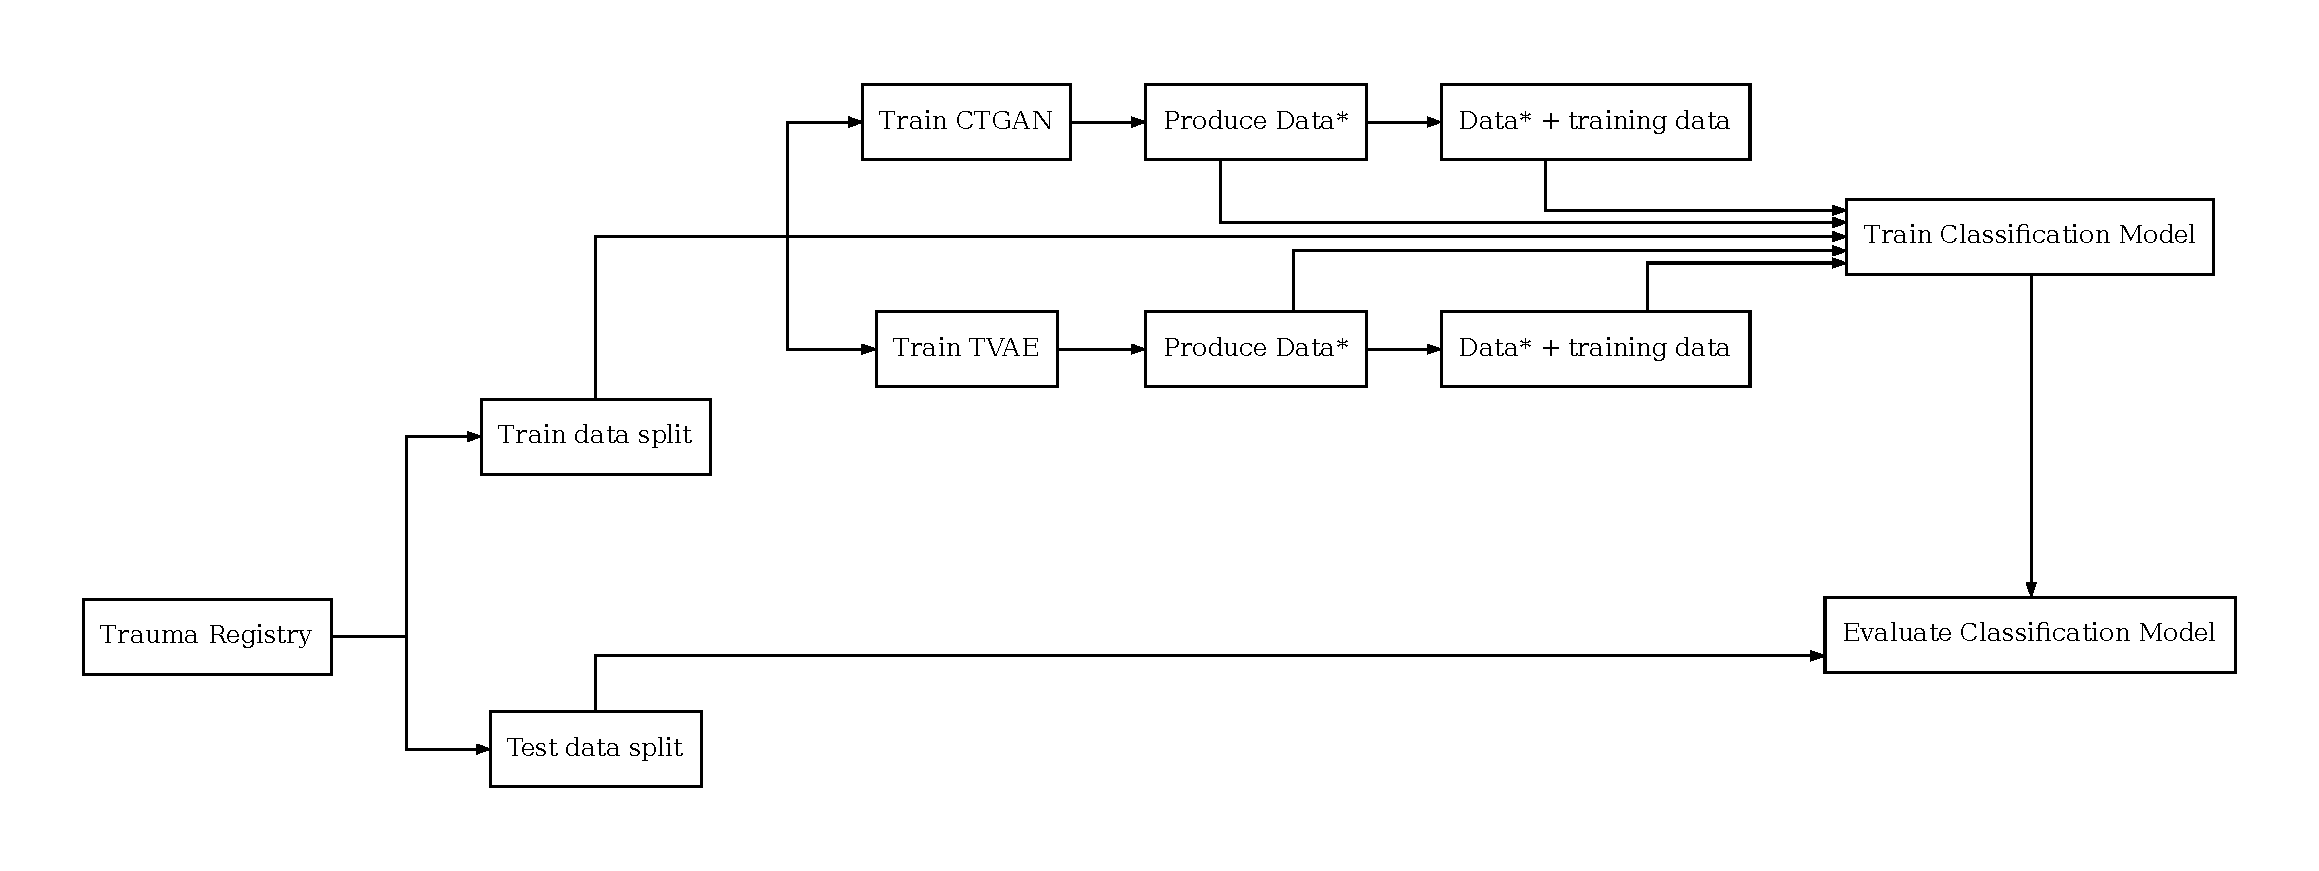
\includegraphics[width=\textwidth]{figures/model_flowchart.pdf}
    \caption{\textbf{Flowchart describing the process of evaluating the synthesising models.}\\
        Process is replicated for each classification model and resample. Each arrow to "Train Classification Model" indicates an individual and separated training/evaluation cycle from the other data inputs.\\
        *Synthetic training data output by a data synthesising model.\\
        \textit{Definition of abbreviations:} CTGAN = Conditional tabular generative adversarial network; TVAE = Triplet based variational autoencoder.}
    \label{fig:modelflowchart}
\end{figure}

%% I think some more work is needed to describe the different sets of models created. In my understanding, you create one set of models for each "synthesiser" and then one set of baseline models. So for Logistic regression you have LRctgan, LRtvae, and LRbl, for random forest RFctgan, RFtvae, and RFbl, and so on. You then compare LRbl with LRctgan and LRbl with LRtvae. Do you also compare LRctgan with LRtvae? Will you calculate a mean delta and compare these, so that you can say if "on avarage" the ctgan performed better than tvae? 
All statistical analyses were performed using Python. The model analyses were conducted by splitting the data into an 80\%-20\% train-test and repeating the process 100 times using random resampling without replacement. The estimated 95\% \acrfull{ci} using $t$-distribution was calculated for \acrfull{auc} as well as the delta values, using all resamples. A significance level at $p$-value $< 0.05$ was set.

The synthesising models were trained on the raw training data from each resample. The synthesising models generated an output dataset with an equal size to the input training data. The classification models were trained on either the pre-processed training data from the resample, the pre-processed output of the synthesising models, or a combination of both (\Cref{fig:modelflowchart}). During each training cycle, the classification models were tested on the pre-processed test data from the train-test split, and the \acrshort{auc} was calculated. This resulted in each classification model being evaluated five times for each resample: using the raw training data, the \acrshort{ctgan} synthetic data, a combination of the raw training data and \acrshort{ctgan} synthetic data, the \acrshort{tvae} synthetic data, and a combination of the raw training data and \acrshort{tvae} synthetic data. Each data input mentioned is referred to as a data group.

The performance of the models was assessed on the test split from each resample and compared using \acrshort{auc}. Additionally, the delta \acrshort{auc} for each model was calculated for each resample. The performance of a classification model was compared both to models within the same data group and to models in different data groups. Finally, the average delta \acrshort{auc} was calculated for each data group and compared to other groups.

Descriptive statistics, including mean, \acrfull{sd}, median, minimum, and maximum for continuous features, and prevalence for categorical features, were calculated. Descriptive statistics were computed for both the baseline and synthetic datasets.

\subsection{Ethical Considerations}
The group under investigation in this study, trauma patients, can be considered a vulnerable population due to the severe outcomes that often result from major trauma, such as disability and death. Thus, special consideration must be given to the ethics of conducting this study. It is important to note that only anonymous registry data was used in this study, and no identifiable personal data was accessible by the authors or the \acrshort{ml} models, this is one of the important measurements taken to reduce possible ethical complications.

In terms of autonomy and non-maleficence, no interventions were made that could potentially harm the patients. The registry on which this study was based, \acrshort{swetrau}, operates under the assumption of presumed consent, meaning that if a patient does not explicitly opt out of being included in the registry, it is assumed that they have consented to participate. While this study poses almost no risk of harm to the study population, the absence of sensitive personal data also reduces the risk of stigmatising a particular group.

The study aligns with the principle of beneficence, as its purpose is to improve clinical models for detecting \acrshortpl{ofi} and improve patient care in the long run. The study provides valuable insights into methods to improve the performance of \acrshort{ml} models in this area.

The ethical considerations associated with synthesising personal data warrant further discussion. If it were possible to generate 100\% anonymous synthesised data, would the same ethical principles apply? Since the synthesised data does not represent actual patients, it is difficult to consider autonomy and justice in this context. However, conducting epidemiological studies on randomly generated or simulated data is typically done without much ethical consideration. There must be a consensus on these ethical considerations before synthesising models can produce highly accurate synthetic data.

In conclusion, the benefits of this study, as measured against the four principles of Beauchamp and Childress (autonomy, non-maleficence, descence, and justice), outweigh the potential risks. The study was approved by the Stockholm Research Ethics Review Board (permits 2021-02541 and 2021-03531).

\section{Results}
\subsection{Patient Characteristics}
\begin{figure}[ht]
    \centering
    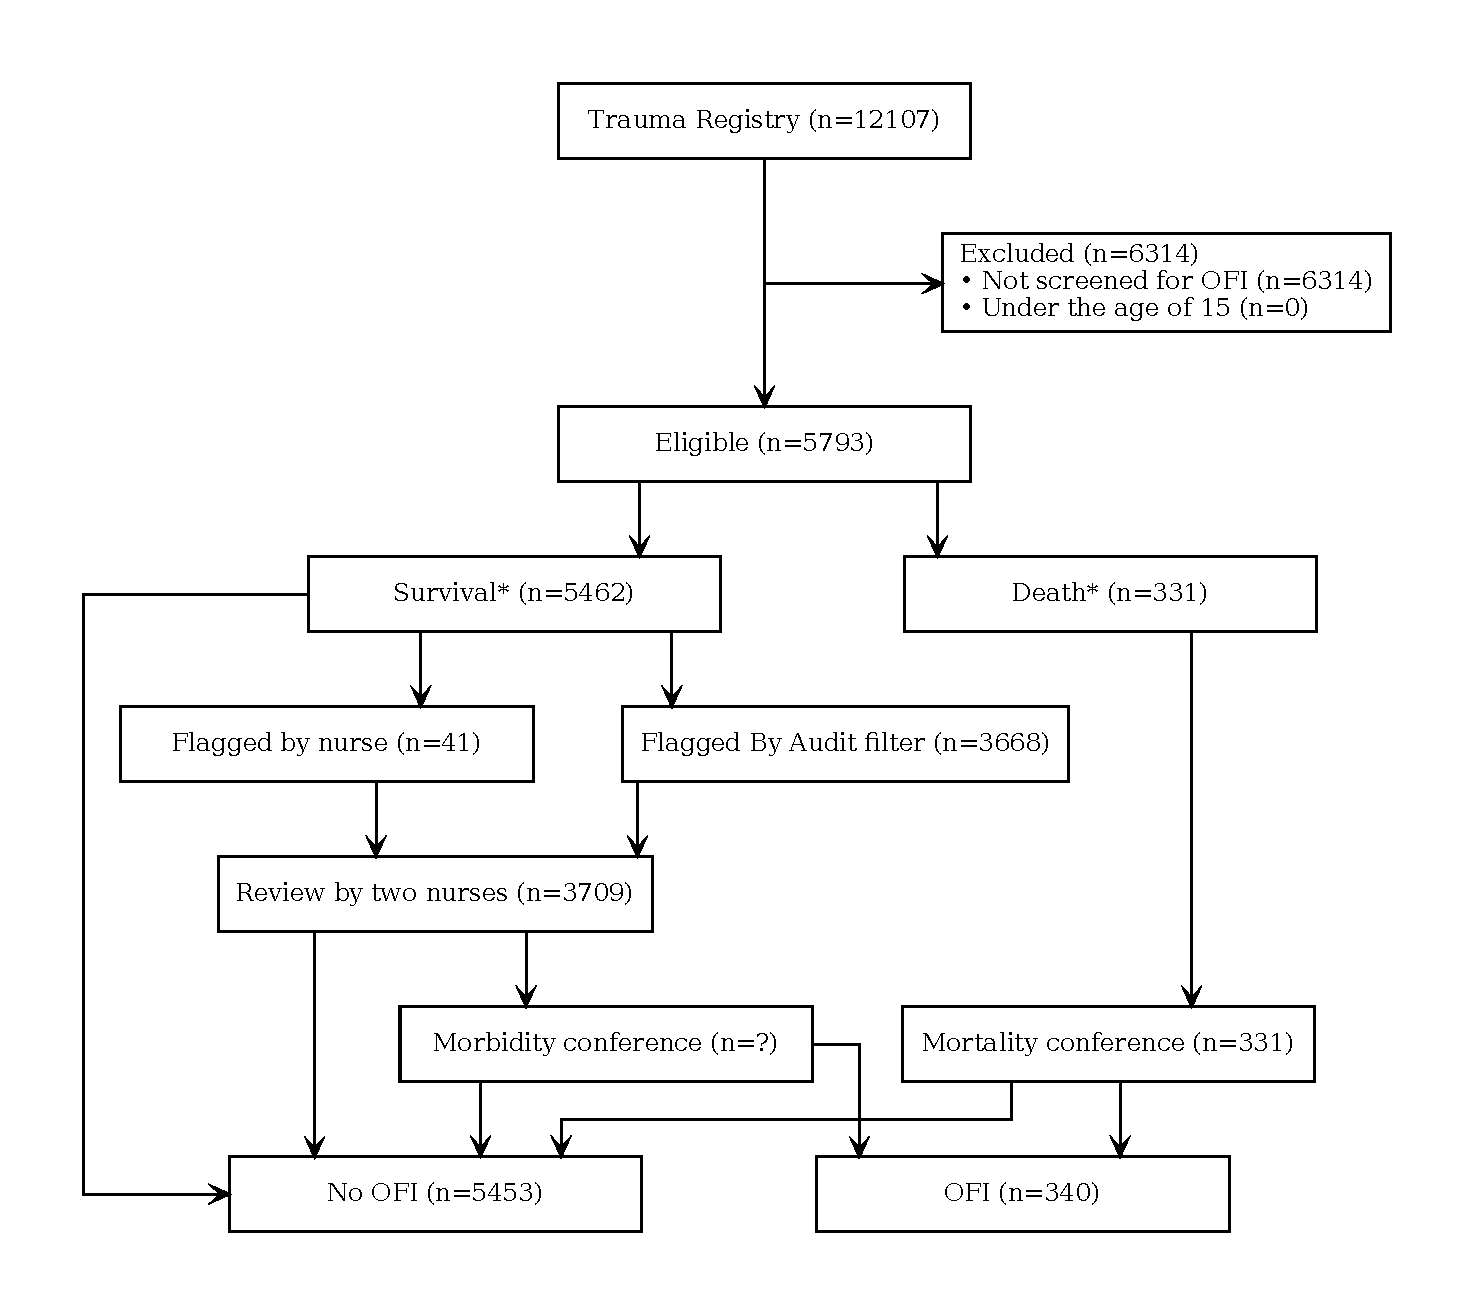
\includegraphics[width=0.85\textwidth]{figures/flowchart.pdf}
    \caption{\textbf{Flowchart describing the exclusions made and including the process to determine a case with \acrshort{ofi}.}\\
        *Defined at 30-days post trauma.\\
        \textit{Definition of abbreviations:} OFI = opportunity for improvement.}
    \label{fig:flowchart}
\end{figure}
During the years 2014 to 2021, a population of \num{12107} trauma patients were identified. For \num{6314} patients were excluded due to not being screened for an \acrshort{ofi} by either audit filters or individual review, zero patients were excluded for being under the age of 15. In total \num{5793} patients were eligible and included in the study. A large majority of these cases, \num{5453} patients, reached the consensus that no \acrshort{ofi} was present while \num{340} patients were deemed to have at least one \acrshort{ofi}. A summarised graph of inclusion and exclusion criteria including the process to an \acrshort{ofi} is seen in \Cref{fig:flowchart}.

\begin{table}[t!]
    \centering
    \renewcommand{\arraystretch}{0.9}
    \caption{\textbf{Patient demographic and clinical characteristics}.\\
        Subdivided by \acrshort{ofi} outcome for ground truth data.}
    \label{tab:tableone}
    \scalebox{0.7}{
        \begin{tabular}{lccc}
            \toprule
                                                          & \textbf{Overall}  & \textbf{No OFI}   & \textbf{OFI}     \\
            \midrule
                                                          & $n=5793$          & $n=5453$          & $n=340$          \\
            \textbf{Age}                                  &                   &                   &                  \\
            \hspace{3mm}Mean (SD)                         & 46 (21)           & 45 (21)           & 50 (22)          \\
            \hspace{3mm}Median [Min, Max]                 & 43 [15, 100]      & 43 [15, 100]      & 50 [15, 97]      \\
            \hspace{3mm}Missing                           & 651 (11\%)        & 617 (11\%)        & 34 (10\%)        \\
            \textbf{Gender}                               &                   &                   &                  \\
            \hspace{3mm}Male                              & 3509 (61\%)       & 3293 (60\%)       & 216 (64\%)       \\
            \hspace{3mm}Female                            & 1633 (28\%)       & 1543 (28\%)       & 90 (26\%)        \\
            \hspace{3mm}Missing                           & 651 (11\%)        & 617 (11\%)        & 34 (10\%)        \\
            \textbf{Dead at 30 days}                      &                   &                   &                  \\
            \hspace{3mm}No                                & 4809 (83\%)       & 4523 (83\%)       & 286 (84\%)       \\
            \hspace{3mm}Yes                               & 331 (6\%)         & 311 (6\%)         & 20 (6\%)         \\
            \hspace{3mm}Missing                           & 653 (11\%)        & 619 (11\%)        & 34 (10\%)        \\
            \textbf{Highest level of care}                &                   &                   &                  \\
            \hspace{3mm}Intensive care unit               & 863 (15\%)        & 761 (14\%)        & 102 (30\%)       \\
            \hspace{3mm}General ward                      & 2002 (35\%)       & 1933 (35\%)       & 69 (20\%)        \\
            \hspace{3mm}Surgical ward                     & 945 (16\%)        & 852 (16\%)        & 93 (27\%)        \\
            \hspace{3mm}ED                                & 1120 (19\%)       & 1106 (20\%)       & 14 (4\%)         \\
            \hspace{3mm}Specialist/Intermediate ward      & 212 (4\%)         & 184 (3\%)         & 28 (8\%)         \\
            \hspace{3mm}Missing                           & 651 (11\%)        & 617 (11\%)        & 34 (10\%)        \\
            \textbf{Injury severity score}                &                   &                   &                  \\
            \hspace{3mm}Mean (SD)                         & 10 (11)           & 10 (11)           & 18 (10)          \\
            \hspace{3mm}Median [Min, Max]                 & 8 [0, 75]         & 5 [0, 75]         & 17 [0, 59]       \\
            \hspace{3mm}Missing                           & 653 (11\%)        & 619 (11\%)        & 34 (10\%)        \\
            \textbf{ED Respiratory Rate}                  &                   &                   &                  \\
            \hspace{3mm}Mean (SD)                         & 23 (20)           & 23 (20)           & 24 (21)          \\
            \hspace{3mm}Median [Min, Max]                 & 18 [0, 99]        & 18 [0, 99]        & 18 [0, 99]       \\
            \hspace{3mm}Missing                           & 683 (12\%)        & 644 (12\%)        & 39 (11\%)        \\
            \textbf{ED Systolic blood pressure}           &                   &                   &                  \\
            \hspace{3mm}Mean (SD)                         & 136 (28)          & 136 (28)          & 135 (31)         \\
            \hspace{3mm}Median [Min, Max]                 & 135 [0, 285]      & 135 [0, 285]      & 135 [0, 237]     \\
            \hspace{3mm}Missing                           & 660 (11\%)        & 626 (11\%)        & 34 (10\%)        \\
            \textbf{ED GCS}                               &                   &                   &                  \\
            \hspace{3mm}Mean (SD)                         & 14 (2)            & 14 (2)            & 14 (2)           \\
            \hspace{3mm}Median [Min, Max]                 & 15 [3, 15]        & 15 [3, 15]        & 15 [3, 15]       \\
            \hspace{3mm}Missing                           & 1008 (17\%)       & 950 (17\%)        & 58 (17\%)        \\
            \textbf{Time to first CT}                     &                   &                   &                  \\
            \hspace{3mm}Mean (SD)                         & 75 (137)          & 74 (137)          & 82 (139)         \\
            \hspace{3mm}Median [Min, Max]                 & 35 [0, 1415]      & 35 [0, 1415]      & 43 [6, 1339]     \\
            \hspace{3mm}Missing                           & 1206 (21\%)       & 1147 (21\%)       & 59 (17\%)        \\
            \textbf{Time to definitive treatment}         &                   &                   &                  \\
            \hspace{3mm}Mean (SD)                         & 263 (354)         & 260 (358)         & 278 (328)        \\
            \hspace{3mm}Median [Min, Max]                 & 110 [0, 2036]     & 104 [0, 2036]     & 154 [9, 1420]    \\
            \hspace{3mm}Missing                           & 4635 (80\%)       & 4453 (82\%)       & 182 (54\%)       \\
            \textbf{Intubated}                            &                   &                   &                  \\
            \hspace{3mm}No                                & 5285 (91\%)       & 4997 (92\%)       & 288 (85\%)       \\
            \hspace{3mm}Yes                               & 508 (9\%)         & 456 (8\%)         & 52 (15\%)        \\
            \hspace{3mm}Missing                           & 0 (0\%)           & 0 (0\%)           & 0 (0\%)          \\
            \textbf{Emergency procedure}                  &                   &                   &                  \\
            \hspace{3mm}Laparotomy                        & 114 (2\%)         & 100 (2\%)         & 14 (4\%)         \\
            \hspace{3mm}Craniotomy                        & 131 (2\%)         & 111 (2\%)         & 20 (6\%)         \\
            \hspace{3mm}Other                             & 787 (14\%)        & 699 (13\%)        & 88 (26\%)        \\
            \hspace{3mm}Radiological intervention         & 51 (\textless1\%) & 29 (\textless1\%) & 22 (6\%)         \\
            \hspace{3mm}Thoracotomy                       & 18 (\textless1\%) & 17 (\textless1\%) & 1 (\textless1\%) \\
            \hspace{3mm}Intracranial pressure measurement & 34 (\textless1\%) & 28 (\textless1\%) & 6 (2\%)          \\
            \hspace{3mm}Revascularisation                 & 22 (\textless1\%) & 15 (\textless1\%) & 7 (2\%)          \\
            \hspace{3mm}Pelvis packing                    & 2 (\textless1\%)  & 2 (\textless1\%)  & 0 (0\%)          \\
            \hspace{3mm}Missing                           & 4634 (80\%)       & 4452 (82\%)       & 182 (54\%)       \\
            \bottomrule
        \end{tabular}
    }
    \caption*{\small Time to first CT and Time to definitive treatment are measured in minutes from arrival at the hospital.\\
        \textit{Definition of abbreviations:} OFI = Opportunity for Improvement; ED = Emergency Department; GCS = Glascow Coma Scale.}
\end{table}

Selected patient characteristics are summarised in \Cref{tab:tableone}. The trauma group as a whole had a mean age of 46 (\acrshort{sd}: 21) while the \acrshort{ofi} and \acrshort{ofi} negative subgroup had a mean age of 50 (\acrshort{sd}: 22) and 45 (\acrshort{sd}: 21) respectively. The majority were male ($n = $ \num{3509}, 61\%) and the overall group had a mortality of 6\% ($n = $ \num{331}). The \acrshort{ofi} group had a higher mean \acrshort{iss} (18 [\acrshort{sd}: 10] vs 10 [\acrshort{sd}: 11]) and were admitted to the intensive care unit more frequently (30\% [$n = $ \num{286}] vs 14\% [$n = $ \num{761}]). Data for emergency procedure was less missing in the \acrshort{ofi} subgroup with 54\% ($n = $ 182) of records missing data compared to 82\% ($n = $ \num{4452}) in the \acrshort{ofi} negative group. Furthermore, the emergency procedure "other" was more common in the \acrshort{ofi} group (26\% [$n = $ \num{88}] vs 13\% [$n = $ \num{699}]).

Selected patient characteristics for the data produced by the synthesising models are presented in \Cref{tab:tableonectgan,tab:tableonetvae} in the appendix.

\subsection{Model Performance}
\begin{table}[ht!]
    \centering
    \renewcommand{\arraystretch}{1.5}
    \caption{\textbf{Model performances}.}
    \label{tab:modelperf}
    \scalebox{0.75}{
        \begin{tabular}{lP{3cm}P{3cm}P{3cm}P{3cm}P{3cm}}
            \toprule
            Model               & Baseline                             & CTGAN                       & TVAE                        & CTGAN + Baseline                     & TVAE + Baseline             \\
            \midrule
            CatBoost            & \textbf{0.789\newline(0.784, 0.794)} & 0.573\newline(0.551, 0.579) & 0.681\newline(0.615, 0.659) & 0.775\newline(0.772, 0.782)          & 0.779\newline(0.771, 0.781) \\\hline
            Extra Trees         & \textbf{0.775\newline(0.771, 0.781)} & 0.611\newline(0.586, 0.611) & 0.596\newline(0.585, 0.622) & 0.763\newline(0.757, 0.768)          & 0.763\newline(0.76, 0.77)   \\\hline
            k-NN                & 0.715\newline(0.71, 0.721)           & 0.541\newline(0.52, 0.545)  & 0.521\newline(0.521, 0.533) & \textbf{0.718\newline(0.711, 0.722)} & 0.686\newline(0.682, 0.695) \\\hline
            LightGBM            & \textbf{0.78\newline(0.778, 0.788)}  & 0.548\newline(0.537, 0.56)  & 0.627\newline(0.587, 0.62)  & 0.769\newline(0.767, 0.776)          & 0.773\newline(0.766, 0.777) \\\hline
            Logistic Regression & \textbf{0.768\newline(0.759, 0.769)} & 0.595\newline(0.58, 0.609)  & 0.669\newline(0.592, 0.643) & 0.747\newline(0.742, 0.754)          & 0.752\newline(0.745, 0.756) \\\hline
            Random forest       & \textbf{0.792\newline(0.787, 0.797)} & 0.638\newline(0.619, 0.639) & 0.643\newline(0.603, 0.636) & 0.783\newline(0.779, 0.788)          & 0.779\newline(0.772, 0.783) \\\hline
            SVM                 & \textbf{0.679\newline(0.668, 0.681)} & 0.508\newline(0.489, 0.514) & 0.66\newline(0.593, 0.64)   & 0.387\newline(0.424, 0.474)          & 0.648\newline(0.641, 0.655) \\\hline
            XGBoost             & \textbf{0.77\newline(0.767, 0.776)}  & 0.578\newline(0.559, 0.588) & 0.697\newline(0.602, 0.657) & 0.749\newline(0.743, 0.754)          & 0.744\newline(0.739, 0.751) \\
            \bottomrule
        \end{tabular}
    }
\end{table}

\begin{figure}[ht!]
    \centering
    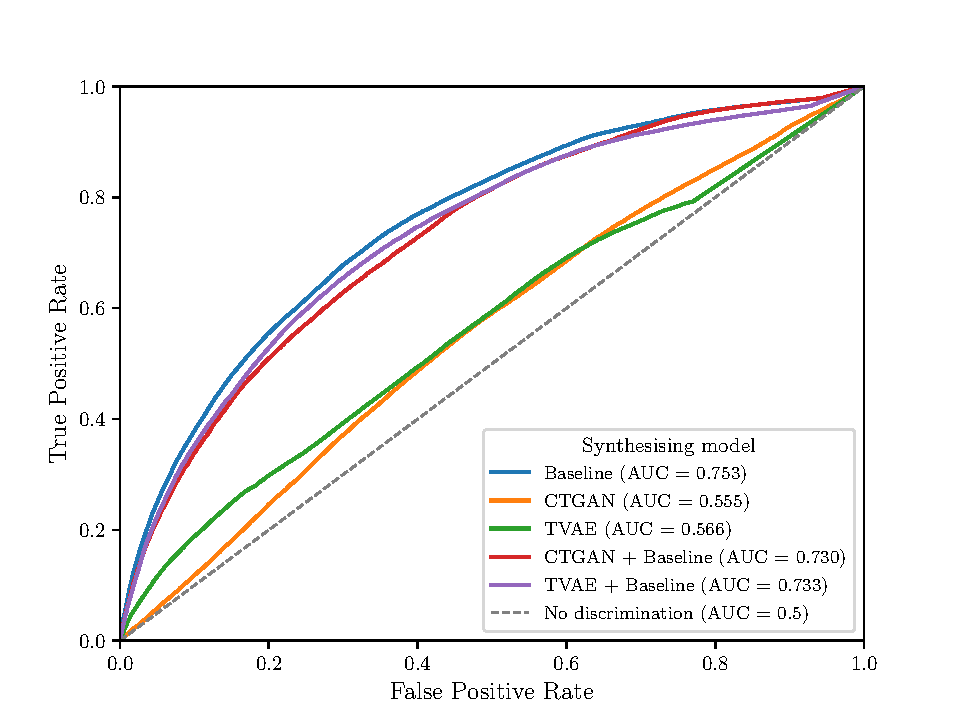
\includegraphics[width=0.85\textwidth]{figures/roc.pdf}
    \caption{\textbf{Receiver operating characteristic curve for synthesising models.}\\
        *Defined at 30-days post trauma.\\
        \textit{Definition of abbreviations:} AUC = \Acrlong{auc}; CTGAN = \Acrlong{ctgan}; TVAE = \Acrlong{tvae}.}
    \label{fig:flowchart}
\end{figure}


\section{Discussion}

\section{Conclusions}

\section*{Contributions}

\section*{Acknowledgement}

\newpage

\singlespacing

\printbibliography

\newpage

\begin{appendices}
    \setcounter{table}{0}
    \renewcommand{\thetable}{A\arabic{table}}

    \setcounter{figure}{0}
    \renewcommand{\thefigure}{A\arabic{figure}}

    \setcounter{secnumdepth}{1}

    \section{Tables}
    \begin{table}[h]
        \centering
        \renewcommand{\arraystretch}{1.2}

        \caption{\textbf{All the currently used audit filters at Karolinska University Hospital.}}
        \label{tab:auditfilters}

        \begin{tabular}{@{}|p{0.85\linewidth}|@{}}
            \hline
            \multicolumn{1}{|c|}{\textbf{Audit filter}}                                                \\\hline
            Systolic blood pressure less than 90                                                       \\\hline
            Glasgow coma scale less than 9 and not intubated                                           \\\hline
            Injury severity score greater than 15 but not admitted to the intensive care unit          \\\hline
            Time to acute intervention more than 60 minutes from arrival to hospital                   \\\hline
            Time to computed tomography more than 30 minutes from arrival to hospital                  \\\hline
            No anticoagulant therapy within 72 hours after traumatic brain injury                      \\\hline
            The presence of cardio-pulmonary resuscitation with thoracotomy                            \\\hline
            The presence of a liver or spleen injury                                                   \\\hline
            Massive transfusion, defined as 10 or more units of packed red blood cells within 24 hours \\\hline
            Other non-defined reason found by first reviewing nurse                                    \\\hline
        \end{tabular}
    \end{table}


    \renewcommand*{\arraystretch}{1.2}
    \begin{longtable}[c]{@{}|l|p{0.55\linewidth}|@{}}
        \caption{\textbf{Predictors used in the development of the \acrlong{ofi} classification and synthesising models.}}%
        \label{tab:predictors}                                                                                          \\
        \hline
        \multicolumn{1}{|c|}{\textbf{SweTrau code}} & \multicolumn{1}{|c|}{\textbf{Description}}                        \\\hline
        \endfirsthead
        %
        \endhead
        %
        AlarmRePrioritised                          & Reprioritisation of trauma code                                   \\\hline
        FirstTraumaDT\_NotDone                      & Trauma CT not done                                                \\\hline
        ISS                                         & Injury Severity Score                                             \\\hline
        NumberOfActions                             & Number of Actions done                                            \\\hline
        NumberOfInjuries                            & Number of injuries                                                \\\hline
        TraumaAlarmAtHospital                       & Type of trauma code criteria                                      \\\hline
        TraumaAlarmCriteria                         & Trauma code at hospital                                           \\\hline
        dt\_alarm\_hosp                             & DT alarm to ED                                                    \\\hline
        dt\_alarm\_scene                            & DT alarm to arrival at scene                                      \\\hline
        dt\_ed\_emerg\_proc                         & DT arrival at ED to emergency procedure                           \\\hline
        dt\_ed\_first\_ct                           & DT arrival at ED to first CT                                      \\\hline
        dt\_ed\_norm\_be                            & DT arrival ED to normalised base excess                           \\\hline
        ed\_be\_art                                 & First base excess at the ED                                       \\\hline
        ed\_be\_art\_NotDone                        & Base excess not taken at ED                                       \\\hline
        ed\_emerg\_proc                             & Emergency procedure at ED                                         \\\hline
        ed\_emerg\_proc\_other                      & Other emergency procedure at ED                                   \\\hline
        ed\_gcs\_motor                              & Motor response according to GCS at ED                             \\\hline
        ed\_gcs\_sum                                & GCS score at ED                                                   \\\hline
        ed\_inr                                     & First Prothrombin time (international normalize ratio)            \\\hline
        ed\_inr\_NotDone                            & Prothrombin time (international normalized ratio) not taken at ED \\\hline
        ed\_intub\_type                             & Intubation type at ED                                             \\\hline
        ed\_intubated                               & Was intubated at ED                                               \\\hline
        ed\_rr\_value                               & Respiratory rate at ED                                            \\\hline
        ed\_sbp\_value                              & Systolic blood pressure at ED                                     \\\hline
        ed\_tta                                     & Trauma team activated                                             \\\hline
        hosp\_dischg\_dest                          & Discharge destination                                             \\\hline
        hosp\_los\_days                             & Total admittance days at hospital                                 \\\hline
        hosp\_vent\_days                            & Total amount of days in a ventilator                              \\\hline
        host\_care\_level                           & Highest level of care                                             \\\hline
        host\_transfered                            & Transferred from/to another hospital                              \\\hline
        host\_vent\_days\_NotDone                   & No days spent on a ventilator                                     \\\hline
        inj\_dominant                               & Dominant type of injury                                           \\\hline
        inj\_intention                              & Injury intention                                                  \\\hline
        inj\_mechanism                              & Dominant injury mechanism                                         \\\hline
        iva\_dagar\_n                               & Total amount of days in the intensive care unit                   \\\hline
        iva\_vardtillfallen\_n                      & Amount of times admitted to the intensive care unit               \\\hline
        pre\_card\_arrest                           & PH cardiac arrest                                                 \\\hline
        pre\_gcs\_motor                             & PH motor response according to GCS                                \\\hline
        pre\_gcs\_sum                               & PH GCS score                                                      \\\hline
        pre\_intub\_type                            & Type of intubation PH                                             \\\hline
        pre\_intubated                              & Was intubated PH                                                  \\\hline
        pre\_provided                               & Level of care given PH                                            \\\hline
        pre\_rr\_value                              & PH Respiratory rate                                               \\\hline
        pre\_sbp\_value                             & PH Systolic blood pressure                                        \\\hline
        pre\_transport                              & Transport type PH                                                 \\\hline
        pt\_Gender                                  & Gender                                                            \\\hline
        pt\_age\_yrs                                & Patient age                                                       \\\hline
        pt\_asa\_preinjury                          & American Society of Anesthesiologists Class pre-injury            \\\hline
        res\_gos\_dischg                            & Glascow outcome score at discharge                                \\\hline
        res\_survival                               & Mortality                                                         \\\hline
        \caption*{\small \textit{Definition of abbreviations:} CT = Computer Tomography; DT = Delta Time; ED = Emergency department; GCS = Glascow Coma Scale; PH = Pre-hospital.}%
    \end{longtable}

    \begin{table}[t!]
        \centering
        \renewcommand{\arraystretch}{0.9}
        \caption{\textbf{Patient demographic and clinical characteristics}.\\
            Subdivided by \acrshort{ofi} outcome for \acrshort{ctgan} data.}
        \label{tab:tableonectgan}
        \scalebox{0.7}{
            \begin{tabular}{lccc}
                \toprule
                                                              & \textbf{Overall}  & \textbf{No OFI}   & \textbf{OFI}     \\
                \midrule
                                                              & $n=5793$          & $n=5293$          & $n=500$          \\
                \textbf{Age}                                  &                   &                   &                  \\
                \hspace{3mm}Mean (SD)                         & 56 (23)           & 56 (23)           & 55 (23)          \\
                \hspace{3mm}Median [Min, Max]                 & 56 [15, 100]      & 56 [15, 100]      & 53 [15, 100]     \\
                \hspace{3mm}Missing                           & 2112 (36\%)       & 1847 (35\%)       & 265 (53\%)       \\
                \textbf{Gender}                               &                   &                   &                  \\
                \hspace{3mm}Female                            & 1566 (27\%)       & 1465 (28\%)       & 101 (20\%)       \\
                \hspace{3mm}Male                              & 2122 (37\%)       & 1988 (38\%)       & 134 (27\%)       \\
                \hspace{3mm}Missing                           & 2105 (36\%)       & 1840 (35\%)       & 265 (53\%)       \\
                \textbf{Dead at 30 days}                      &                   &                   &                  \\
                \hspace{3mm}No                                & 3577 (62\%)       & 3350 (63\%)       & 227 (45\%)       \\
                \hspace{3mm}Yes                               & 121 (2\%)         & 113 (2\%)         & 8 (2\%)          \\
                \hspace{3mm}Missing                           & 2095 (36\%)       & 1830 (35\%)       & 265 (53\%)       \\
                \textbf{Highest level of care}                &                   &                   &                  \\
                \hspace{3mm}General ward                      & 2041 (35\%)       & 1928 (36\%)       & 113 (23\%)       \\
                \hspace{3mm}Intensive care unit               & 842 (15\%)        & 780 (15\%)        & 62 (12\%)        \\
                \hspace{3mm}ED                                & 410 (7\%)         & 385 (7\%)         & 25 (5\%)         \\
                \hspace{3mm}Surgical ward                     & 334 (6\%)         & 305 (6\%)         & 29 (6\%)         \\
                \hspace{3mm}Specialist/Intermediate ward      & 67 (1\%)          & 62 (1\%)          & 5 (1\%)          \\
                \hspace{3mm}Missing                           & 2099 (36\%)       & 1833 (35\%)       & 266 (53\%)       \\
                \textbf{Injury severity score}                &                   &                   &                  \\
                \hspace{3mm}Mean (SD)                         & 7 (9)             & 7 (9)             & 8 (9)            \\
                \hspace{3mm}Median [Min, Max]                 & 5 [0, 75]         & 5 [0, 75]         & 8 [0, 74]        \\
                \hspace{3mm}Missing                           & 2116 (37\%)       & 1851 (35\%)       & 265 (53\%)       \\
                \textbf{ED Respiratory Rate}                  &                   &                   &                  \\
                \hspace{3mm}Mean (SD)                         & 27 (24)           & 27 (23)           & 28 (24)          \\
                \hspace{3mm}Median [Min, Max]                 & 21 [4, 99]        & 21 [4, 99]        & 22 [6, 99]       \\
                \hspace{3mm}Missing                           & 2311 (40\%)       & 2025 (38\%)       & 286 (57\%)       \\
                \textbf{ED Systolic blood pressure}           &                   &                   &                  \\
                \hspace{3mm}Mean (SD)                         & 148 (36)          & 148 (36)          & 141 (35)         \\
                \hspace{3mm}Median [Min, Max]                 & 143 [0, 285]      & 143 [0, 285]      & 138 [0, 274]     \\
                \hspace{3mm}Missing                           & 2238 (39\%)       & 1960 (37\%)       & 278 (56\%)       \\
                \textbf{ED GCS}                               &                   &                   &                  \\
                \hspace{3mm}Mean (SD)                         & 21 (32)           & 21 (32)           & 22 (24)          \\
                \hspace{3mm}Median [Min, Max]                 & 15 [3, 999]       & 15 [3, 999]       & 15 [3, 121]      \\
                \hspace{3mm}Missing                           & 2102 (36\%)       & 1839 (35\%)       & 263 (53\%)       \\
                \textbf{Time to first CT}                     &                   &                   &                  \\
                \hspace{3mm}Mean (SD)                         & 51 (80)           & 50 (79)           & 58 (91)          \\
                \hspace{3mm}Median [Min, Max]                 & 29 [0, 1033]      & 29 [0, 1033]      & 34 [2, 750]      \\
                \hspace{3mm}Missing                           & 2477 (43\%)       & 2167 (41\%)       & 310 (62\%)       \\
                \textbf{Time to definitive treatment}         &                   &                   &                  \\
                \hspace{3mm}Mean (SD)                         & 314 (294)         & 317 (298)         & 285 (245)        \\
                \hspace{3mm}Median [Min, Max]                 & 267 [1, 1727]     & 267 [1, 1727]     & 266 [18, 1311]   \\
                \hspace{3mm}Missing                           & 4925 (85\%)       & 4490 (85\%)       & 435 (87\%)       \\
                \textbf{Intubated}                            &                   &                   &                  \\
                \hspace{3mm}No                                & 5490 (95\%)       & 5025 (95\%)       & 465 (93\%)       \\
                \hspace{3mm}Yes                               & 303 (5\%)         & 268 (5\%)         & 35 (7\%)         \\
                \hspace{3mm}Missing                           & 0 (0\%)           & 0 (0\%)           & 0 (0\%)          \\
                \textbf{Emergency procedure}                  &                   &                   &                  \\
                \hspace{3mm}Laparotomy                        & 242 (4\%)         & 225 (4\%)         & 17 (3\%)         \\
                \hspace{3mm}Thoracotomy                       & 134 (2\%)         & 117 (2\%)         & 17 (3\%)         \\
                \hspace{3mm}Other                             & 32 (\textless1\%) & 32 (\textless1\%) & 0 (0\%)          \\
                \hspace{3mm}Pelvis packing                    & 117 (2\%)         & 111 (2\%)         & 6 (1\%)          \\
                \hspace{3mm}Radiological intervention         & 68 (1\%)          & 66 (1\%)          & 2 (\textless1\%) \\
                \hspace{3mm}Intracranial pressure measurement & 48 (\textless1\%) & 44 (\textless1\%) & 4 (\textless1\%) \\
                \hspace{3mm}Craniotomy                        & 44 (\textless1\%) & 39 (\textless1\%) & 5 (1\%)          \\
                \hspace{3mm}Revascularisation                 & 83 (1\%)          & 79 (1\%)          & 4 (\textless1\%) \\
                \hspace{3mm}Missing                           & 5025 (87\%)       & 4580 (87\%)       & 445 (89\%)       \\
                \bottomrule
            \end{tabular}
        }
        \caption*{\small Time to first CT and Time to definitive treatment are measured in minutes from arrival at the hospital.\\
            \textit{Definition of abbreviations:} OFI = Opportunity for Improvement; ED = Emergency Department; GCS = Glascow Coma Scale.}
    \end{table}

    \begin{table}[t!]
        \centering
        \renewcommand{\arraystretch}{0.9}
        \caption{\textbf{Patient demographic and clinical characteristics}.\\
            Subdivided by \acrshort{ofi} outcome for \acrshort{tvae} data.}
        \label{tab:tableonetvae}
        \scalebox{0.7}{
            \begin{tabular}{lccc}
                \toprule
                                                              & \textbf{Overall}  & \textbf{No OFI}   & \textbf{OFI}  \\
                \midrule
                                                              & $n=5894$          & $n=5793$          & $n=101$       \\
                \textbf{Age}                                  &                   &                   &               \\
                \hspace{3mm}Mean (SD)                         & 51 (26)           & 51 (26)           & 50 (20)       \\
                \hspace{3mm}Median [Min, Max]                 & 47 [15, 100]      & 47 [15, 100]      & 47 [15, 92]   \\
                \hspace{3mm}Missing                           & 360 (6\%)         & 360 (6\%)         & 0 (0\%)       \\
                \textbf{Gender}                               &                   &                   &               \\
                \hspace{3mm}Male                              & 4808 (82\%)       & 4707 (81\%)       & 101 (100\%)   \\
                \hspace{3mm}Female                            & 727 (12\%)        & 727 (13\%)        & 0 (0\%)       \\
                \hspace{3mm}Missing                           & 359 (6\%)         & 359 (6\%)         & 0 (0\%)       \\
                \textbf{Dead at 30 days}                      &                   &                   &               \\
                \hspace{3mm}No                                & 5224 (89\%)       & 5128 (89\%)       & 96 (95\%)     \\
                \hspace{3mm}Yes                               & 311 (5\%)         & 306 (5\%)         & 5 (5\%)       \\
                \hspace{3mm}Missing                           & 359 (6\%)         & 359 (6\%)         & 0 (0\%)       \\
                \textbf{Highest level of care}                &                   &                   &               \\
                \hspace{3mm}Intensive care unit               & 1416 (24\%)       & 1321 (23\%)       & 95 (94\%)     \\
                \hspace{3mm}General ward                      & 2099 (36\%)       & 2099 (36\%)       & 0 (0\%)       \\
                \hspace{3mm}Surgical ward                     & 1120 (19\%)       & 1114 (19\%)       & 6 (6\%)       \\
                \hspace{3mm}ED                                & 883 (15\%)        & 883 (15\%)        & 0 (0\%)       \\
                \hspace{3mm}Specialist/Intermediate ward      & 14 (\textless1\%) & 14 (\textless1\%) & 0 (0\%)       \\
                \hspace{3mm}Missing                           & 362 (6\%)         & 362 (6\%)         & 0 (0\%)       \\
                \textbf{Injury severity score}                &                   &                   &               \\
                \hspace{3mm}Mean (SD)                         & 11 (10)           & 10 (10)           & 32 (7)        \\
                \hspace{3mm}Median [Min, Max]                 & 9 [0, 71]         & 9 [0, 71]         & 32 [10, 45]   \\
                \hspace{3mm}Missing                           & 366 (6\%)         & 366 (6\%)         & 0 (0\%)       \\
                \textbf{ED Respiratory Rate}                  &                   &                   &               \\
                \hspace{3mm}Mean (SD)                         & 24 (20)           & 24 (21)           & 22 (3)        \\
                \hspace{3mm}Median [Min, Max]                 & 18 [5, 99]        & 18 [5, 99]        & 23 [14, 25]   \\
                \hspace{3mm}Missing                           & 896 (15\%)        & 878 (15\%)        & 18 (18\%)     \\
                \textbf{ED Systolic blood pressure}           &                   &                   &               \\
                \hspace{3mm}Mean (SD)                         & 139 (21)          & 139 (21)          & 125 (31)      \\
                \hspace{3mm}Median [Min, Max]                 & 143 [0, 222]      & 143 [0, 222]      & 129 [54, 173] \\
                \hspace{3mm}Missing                           & 451 (8\%)         & 447 (8\%)         & 4 (4\%)       \\
                \textbf{ED GCS}                               &                   &                   &               \\
                \hspace{3mm}Mean (SD)                         & 20 (20)           & 20 (20)           & 14 (2)        \\
                \hspace{3mm}Median [Min, Max]                 & 15 [3, 105]       & 15 [3, 105]       & 14 [5, 16]    \\
                \hspace{3mm}Missing                           & 362 (6\%)         & 362 (6\%)         & 0 (0\%)       \\
                \textbf{Time to first CT}                     &                   &                   &               \\
                \hspace{3mm}Mean (SD)                         & 45 (32)           & 45 (31)           & 54 (48)       \\
                \hspace{3mm}Median [Min, Max]                 & 33 [0, 330]       & 32 [0, 330]       & 39 [15, 282]  \\
                \hspace{3mm}Missing                           & 1050 (18\%)       & 1050 (18\%)       & 0 (0\%)       \\
                \textbf{Time to definitive treatment}         &                   &                   &               \\
                \hspace{3mm}Mean (SD)                         & 244 (343)         & 256 (351)         & 67 (20)       \\
                \hspace{3mm}Median [Min, Max]                 & 84 [0, 1393]      & 87 [0, 1393]      & 65 [27, 119]  \\
                \hspace{3mm}Missing                           & 4294 (73\%)       & 4294 (74\%)       & 0 (0\%)       \\
                \textbf{Intubated}                            &                   &                   &               \\
                \hspace{3mm}No                                & 5269 (89\%)       & 5264 (91\%)       & 5 (5\%)       \\
                \hspace{3mm}Yes                               & 625 (11\%)        & 529 (9\%)         & 96 (95\%)     \\
                \hspace{3mm}Missing                           & 0 (0\%)           & 0 (0\%)           & 0 (0\%)       \\
                \textbf{Emergency procedure}                  &                   &                   &               \\
                \hspace{3mm}Other                             & 462 (8\%)         & 430 (7\%)         & 32 (32\%)     \\
                \hspace{3mm}Intracranial pressure measurement & 606 (10\%)        & 584 (10\%)        & 22 (22\%)     \\
                \hspace{3mm}Radiological intervention         & 52 (\textless1\%) & 52 (\textless1\%) & 0 (0\%)       \\
                \hspace{3mm}Craniotomy                        & 309 (5\%)         & 299 (5\%)         & 10 (10\%)     \\
                \hspace{3mm}Revascularisation                 & 6 (\textless1\%)  & 6 (\textless1\%)  & 0 (0\%)       \\
                \hspace{3mm}Missing                           & 4459 (76\%)       & 4422 (76\%)       & 37 (37\%)     \\
                \bottomrule
            \end{tabular}
        }
        \caption*{\small Time to first CT and Time to definitive treatment are measured in minutes from arrival at the hospital.\\
            \textit{Definition of abbreviations:} OFI = Opportunity for Improvement; ED = Emergency Department; GCS = Glascow Coma Scale.}
    \end{table}
\end{appendices}

\section*{Projektredogörelse}
\setstretch{1.45}

\subsection{B)}

\begin{figure}[ht]
    \centering
    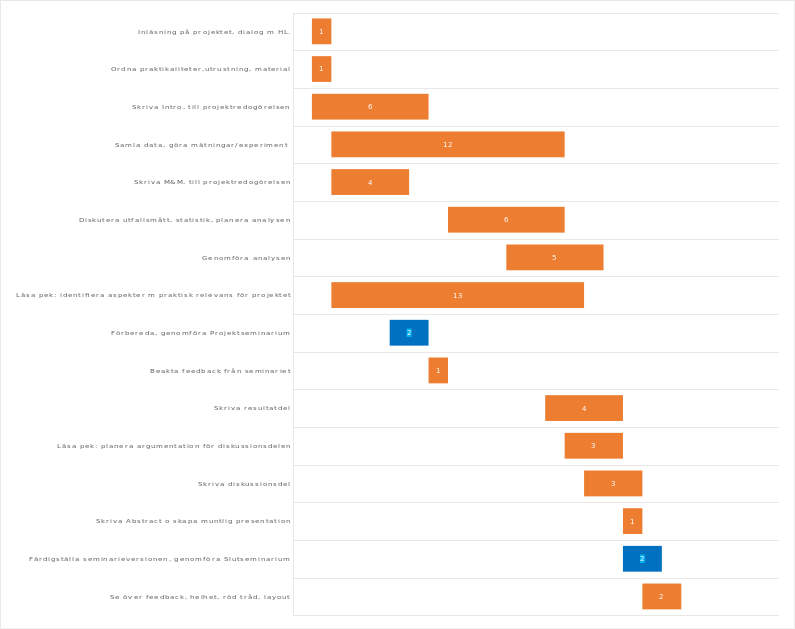
\includegraphics[width=0.75\textwidth]{figures/gant.png}
\end{figure}

Projektet har flytit på bra, all data var redan färdig insamlad innan jag börja. I dagsläget, som det ses i texten, är den deskreptiva analysen på populationen klar. Modellerna (både klassifikation och syntes modellerna) håller på byggas. Det antas att de kommer ta ungefär 3 dagar att köra alla modeller.

Jag tänker presentera den deskreptiva analysen såsom det syns ovan. Huvud resultaten kommer presenteras i tabeller, en tabell för rena prestandan och seperata tabeller för alla delta värden. Möjligtvis att ROC kurvor kommer skapas. Hela metoden är klar och står ovan i texten.

\subsection{C)}
Min reservplan är att testa metoderna på simplare modeller som jag har använt innan och vet funkar. Klassifikationsmodellerna vet vi funkar sedan innan. Det som kan strulas är syntesmodellerna då de är tyngre och har inte använts inom gruppen innan. Vi kan använda äldre syntesmodellern, t.ex. Synthetic Minority Over-sampling Technique (SMOTE) och Adaptive Synthetic (ADASYN). Dessa används inte i uppsatsen nu då de inte kan generera helt ny data och därmed klassifieras inte som en äkta "syntesmodell". Jag tror ej detta kommer behövas då preliminär resultat visar att vi kommer få resultat och att allt går enligt planen.

\end{document}
